\section{RunOff Application}
For the final sprint the focus was on getting the application to communicate with the matchmaking server to allow two users to connect and compete against each other. The goal was to create a prototype with the functionality most crucial to the projects original vision.

\subsection{User Interface} 
The user interface was re-designed such that when a user has selected a route to run they will be directed back to the matchmaking screen and a small toast is displayed informing the user of the name of the chosen route. The user can then press the "matchmake" button to start the matchmaking process while also navigating to the Run Progress activity. For a user to start a competitive run at this point the flow is as shown in \ref{fig:userflow}

\begin{figure}[ht]
\begin{center}
 \caption{User Interface Flow}
 \label{fig:userflow}
 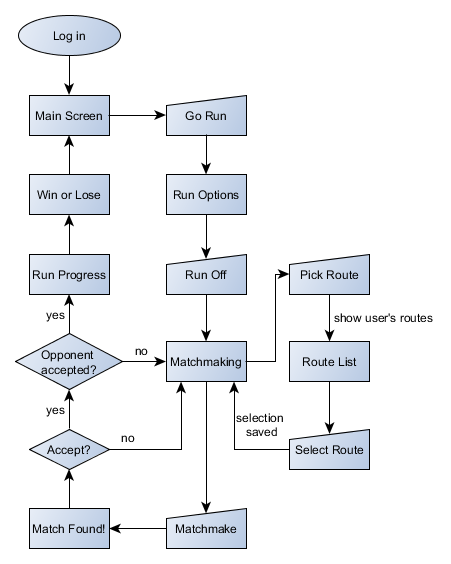
\includegraphics[scale=0.4]{img/runappflow.png}
\end{center}
\end{figure}

The main visual changes from the previous design of the Run Progress activity is a pop-up prompting the user to accept or decline a match as well as a toast counting down until the start of the race when both users have accepted. Once the race has started the Run Progress activity will start sending the position of the runner to the matchmaking server and listening for the position of the opponent. The progress of the opponent is shown relative to the user's own route such that if the opponent is 25\% done with their route, a marker will show up on the user's map indicating where the opponent would be on the user's route. The matchmaking server will at some point determine a winner and when the result is received a toast will be made indicating to the user if they are the winner or not.

The interface of the Run Progress activity should now look like \ref{fig:mapMockV2}

\begin{figure}[ht]
\begin{center}
 \caption{Run Progress Mock-up}
 \label{fig:mapMockV2}
 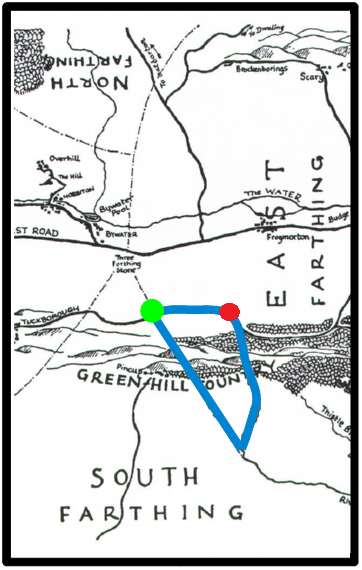
\includegraphics[scale=0.4]{img/mapMockV2.png}
\end{center}
\end{figure}

\subsection{Implementation}
